\pagebreak
\section{Cursograma de Cobranzas}
La empresa posee distintas formas de cobros, las cuales varian con el cliente. Algunas clientes pagan a traves de una cuenta corriente con una transferencia, otros con cheque o efectivo. A determinados clientes se les envía un cobrador mientras que muchos otros no.
Por simplicidad, en este caso se describe el caso en el cual el cliente se acerca a la empresa al sector de finanzas a entregar los valores (cheques o efectivo).

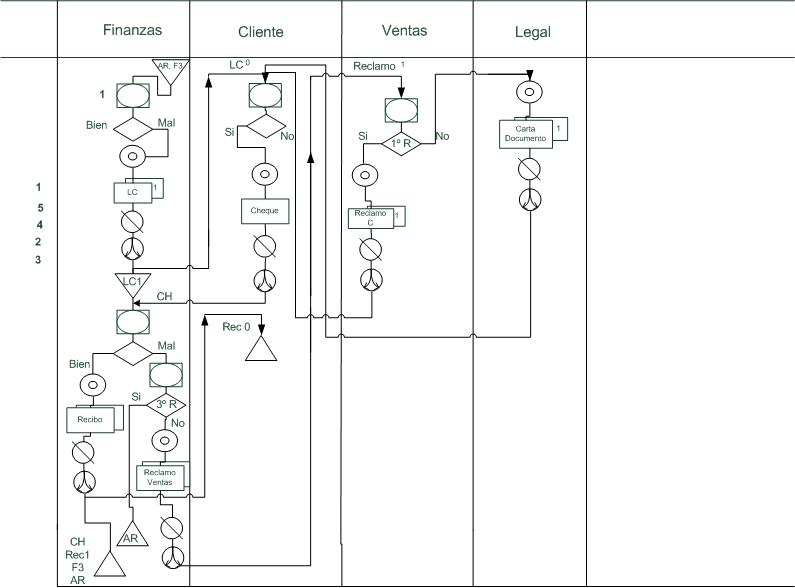
\includegraphics[scale=0.7]{Empresa/Circuitos/Cobranzas/cursograma-manual-cobranzas.jpg}

\pagebreak
\section{Procedimiento de Cobranzas}
\begin{enumerate}
  \item El sector de finanzas ejecuta un reporte en el sistema, el cual trae todas las facturas que vencen a la fecha. De ellas selecciona aquellas que no han sido pagadas. Esta tarea se realiza todos los días.
  \item Por cada factura vencida que no este paga, emite un reclamo del pago por duplicado, con una fecha de vencimiento de pago. El primero lo firma y se lo envía al cliente. El otro lo archiva para que quede constancia del reclamo.
  \item El cliente recibe el reclamo o carta de documento, y en caso de pagar, confecciona un cheque para realizar el mismo y lo envia al sector de finanzas.
  \item Finanzas en caso de recibir el cheque, revisa que corresponda con la cantidad a pagar y que este correctamente confeccionado. Si este esta correcto, emite un recibo por duplicado, firma el original y se lo entrega al cliente. Finalmente, archiva el cheque, la factura por triplicado, el duplicado del reclamo y registra en el sistema el pago de la factura.
  Si el cliente no paga, emite un reclamo a ventas y se lo envia a dicho sector. Si ya es la tercera vez que el cliente no paga, archiva los documentos utilizados y asienta en el sistema la falta de pago en la cuenta "pérdidas". 
  \item Si el cliente no realiza el pago se confecciona un reclamo de Ventas que se firma y se envia al sector de Ventas.
  \item Ventas recibe el reclamo y si es la primera vez que se recibe un reclamo emite un segundo reclamo al cliente por duplicado. Firma el original y lo envia al cliente con una fecha límite para el pago. Si no es la primera vez que recibe un reclamo de finanzas, avisa de al sector legal de la falta de pago del cliente de manera informal(mail, llamado telefónico).
  \item El sector de legal, una vez notificado de la falta de pago del cliente, emite una carta de documento, intimando al cliente a pagar las facturas que debe. La carta de documento es enviada al domicilio legal del cliente de forma tal que quede notificado.
\end{enumerate}

\pagebreak
\section{Manual del Cursograma de Cobranzas}


\pagebreak
\section{Formularios de Cobranzas}
\subsection{Formulario1}
imagen
\begin{itemize}
  \item \textbf{Objetivo:}
  \item \textbf{Alcance:}
  \item \textbf{Emisor:}
  \item \textbf{Cantidad de Copias Emitidas:}
  \item \textbf{Sector receptor:}
 \end{itemize}
\subsubsection{Descripci\'on campos del Formulario1}

\subsection{Formulario2}
imagen
\begin{itemize}
  \item \textbf{Objetivo:}
  \item \textbf{Alcance:}
  \item \textbf{Emisor:}
  \item \textbf{Cantidad de Copias Emitidas:}
  \item \textbf{Sector receptor:}
 \end{itemize}
\subsubsection{Descripci\'on campos del Formulario2}

\pagebreak
\section{Normas de Control Interno de Cobranzas}
